\documentclass[tikz]{standalone}
\usepackage{verbatim}
\begin{document}
\newlength\yearposx
\begin{tikzpicture}[scale=0.57] % timeline 1990-2010->
    % define coordinates (begin, used, end, arrow)
    \foreach \x in {1990,1992,2000,2002,2004,2005,2008,2009,2010,2011}{
        \pgfmathsetlength\yearposx{(\x-1990)*1cm};
        \coordinate (y\x)   at (\yearposx,0);
        \coordinate (y\x t) at (\yearposx,+3pt);
        \coordinate (y\x b) at (\yearposx,-3pt);
    }
    % draw horizontal line with arrow
    \draw [->] (y1990) -- (y2011);
    % draw ticks
   \foreach \x in {1992,2000,2002,2004,2005,2008,2009}
        \draw (y\x t) -- (y\x b);
    % annotate
    \foreach \x in {1992,2002,2005,2009}
        \node at (y\x) [below=3pt] {\x};
    \foreach \x in {2000,2004,2008}
        \node at (y\x) [above=3pt] {\x};
    \begin{comment}
    % for use in beamer class
    \only<2>    {\fill      (y1992) circle (5pt);}
    \only<3-5>  {\fill      (y2000) circle (5pt);}
    \only<4-5>  {\fill      (y2002) circle (5pt);}
    \only<5>    {\fill[red] (y2004) circle (5pt);}
    \only<6>    {\fill      (y2005) circle (5pt);}
    \only<7>    {\fill[red] (y2005) circle (5pt);}
    \only<8-11> {\fill      (y2008) circle (5pt);}
    \only<11>   {\fill      (y2009) circle (5pt);}
    \end{comment}
\end{tikzpicture}
\end{document}